\documentclass{article}
\usepackage{tikz}
\pagestyle{empty}

\begin{document}

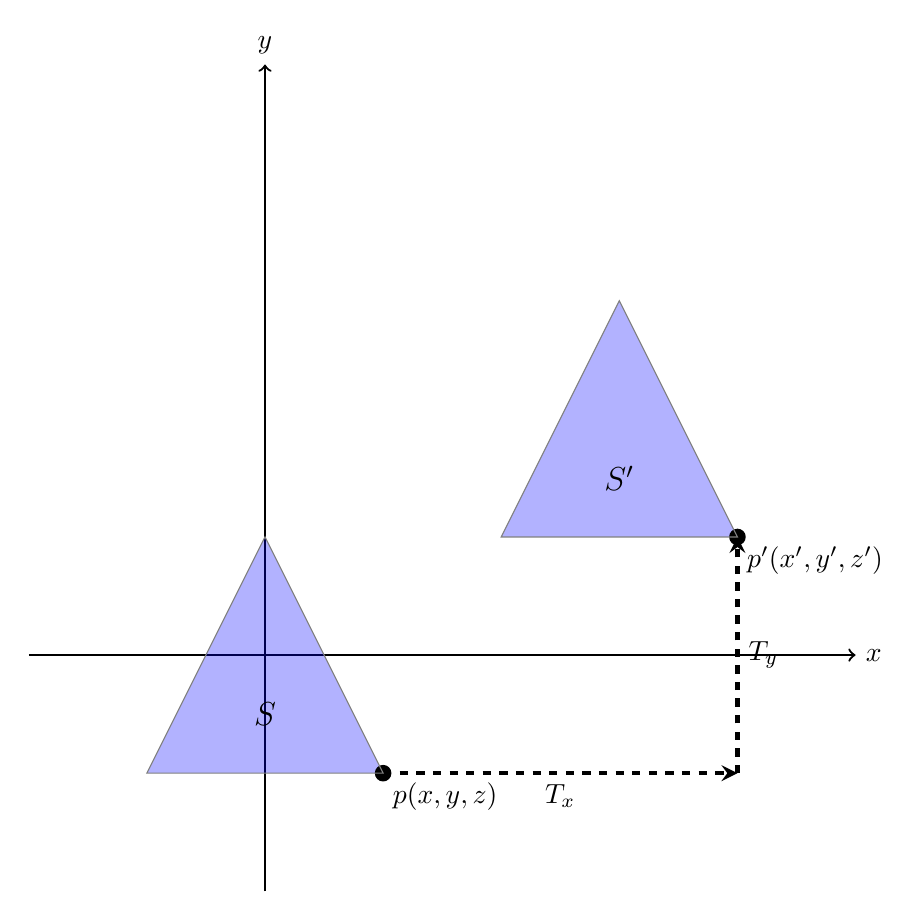
\begin{tikzpicture}[scale=1.5]
    % Draw axes
    \draw[thick, ->] (-2,0) -- (5,0) node[right] {$x$};
    \draw[thick, ->] (0,-2) -- (0,5) node[above] {$y$};
    
    % Draw triangles
    \fill[blue, opacity=0.3] (-1,-1) -- (1,-1) -- (0,1) -- cycle;
    \node at (0, -0.5) {\large $S$}; % Using $...$ to enter math mode for proper rendering
    \fill[blue, opacity=0.3] (2,1) -- (4,1) -- (3,3) -- cycle;
    \node at (3, 1.5) {\large $S'$}; % Using $...$ to enter math
    
    % Draw points
    \fill (1,-1) circle (2pt) node[below right] {$p(x,y,z)$};
    \fill (4,1) circle (2pt) node[below right] {$p'(x',y',z')$};
    
    % Draw translation arrows
    \draw[->, thick, black, dashed, >=stealth, line width=1.5pt] (1,-1) -- (4,-1) node[midway, below] {$T_x$};
    \draw[->, thick, black, dashed, >=stealth, line width=1.5pt] (4,-1) -- (4,1) node[midway, right] {$T_y$};
    
    % Draw triangles' outlines
    \draw[gray] (-1,-1) -- (1,-1) -- (0,1) -- cycle;
    \draw[gray] (2,1) -- (4,1) -- (3,3) -- cycle;
\end{tikzpicture}

\end{document}

